
\documentclass[../main.tex]{subfiles}
\begin{document}

\chapter{Background}
\label{ch:background}

\section{Mathematical backgound}
In this section, we will introduce the basic mathematic notions needed to understand the methods proposed in \cite{hofer_densified_2021, moschella_relative_2022} as well as the ones described in Chapter \ref{ch:methods}.  For that, I will mainly follow \cite{edelsbrunner_computational_2010} \todo{add the rest} as a reference.

\subsection{Simplicial complex}
As we discussed in the introduction, we would want to analyze the characteristics of the underlying manifold from which our dataset has been sampled. Therefore, our objective will be to give some structure to our dataset from which we can assess the aforementioned topological properties.

One way to represent some topological spaces is through decomposition in simpler pieces. A decomposition is called a complex if its pieces are topologically simpler and its intersections are pieces of the same type but lower dimensional \cite{edelsbrunner_computational_2010}. There is a great variety of complexes with different levels of abstraction. However, we will focus on simplicial complexes, which can represent most of the spaces that arise in data science, and they are especially convenient from a computational perspective.\\

Simplicial complexes can be observed from a geometric and combinatorial point of view. First, we will study their definition and main properties from the geometric perspective. For that, reviewing the following affine geometry concepts will be helpful. 

\begin{definition}
A subset of points $\{u_0, u_1, ..., u_k\} \subseteq \mathbb{R}^d$ is \emph{affinely independent} if the vectors $\{\overrightarrow{u_0u_1}, ..., \overrightarrow{u_0u_k}\}$ are linearly independent.
\end{definition}

\begin{definition}
\begin{sloppypar}
We say that $x \in \mathbb{R}^d$ is a \emph{convex combination} of the points ${u_0, u_1, ..., u_k}$ if $x = \sum_{i=0}^{k} \lambda_i u_i$ with $\lambda_i \geq 0 \ \text{ for all } i \in \{0,...,k\}$ and $\sum_{i=0}^{k} \lambda_i = 1$.
\end{sloppypar}
\end{definition}

\begin{definition}
\begin{sloppypar}
We call \emph{convex hull} of $u_0, u_1, ..., u_k$, denoted by ${\text{conv}\{u_0, u_1, ..., u_k\}}$, to the set of all convex combinations of the given points.
\end{sloppypar}
\end{definition}
Using this set, we can define our decomposition pieces as follows:

\begin{definition}
A \emph{$k$\textit{-simplex}} $\sigma$ in $\mathbb{R}^d$ with $d \geq k$ is the convex hull of $k+1$ affinely independent points $u_0, u_1, ..., u_k \in \mathbb{R}^d$, i.e.,
$\sigma \coloneqq \text{conv}\{u_0, u_1, ..., u_k\}$.
\end{definition}

We say that the $k$-simplex $\sigma$ has dimension $k$ and we call \emph{vertex of $\sigma$} to the points $u_0, u_1, ..., u_k$.

\begin{figure}[h]
\centering
\begin{subfigure}[b]{0.2\textwidth}
\centering
   
\begin{tikzpicture}[thick, scale=0.7]
    	\tikzstyle{point}=[circle,thick,draw=black,fill=black,inner sep=0pt,minimum width=4pt,minimum height=4pt]
    	\node (a)[point] at (0,0) {};
    \end{tikzpicture}
    \caption{0-simplex}\label{ref:0simp}
\end{subfigure}
\begin{subfigure}[b]{0.2\textwidth}
\centering
	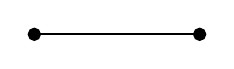
\begin{tikzpicture}[thick, scale=0.7]
    	\tikzstyle{point}=[circle,thick,draw=black,fill=black,inner sep=0pt,minimum width=4pt,minimum height=4pt]
    	\node (a)[point] at (0,0) {};
    	\node (b)[point] at (3,0) {};
 
    	\draw (a.center) -- (b.center) --cycle;
	\end{tikzpicture}
	\caption{1-simplex}\label{ref:1simp}
\end{subfigure}\hspace{0.05\textwidth}
\begin{subfigure}[b]{0.2\textwidth}
\centering
	\begin{tikzpicture}[thick, scale=3]
    	\tikzstyle{point}=[circle,thick,draw=black,fill=black,inner sep=0pt,minimum width=4pt,minimum height=4pt]
    	\coordinate (a) at (0,0);
    	\coordinate (b) at (1,0);
    	\coordinate (c) at (0.6,0.5);

    	\draw[fill=greeo,opacity=0.6] (a) -- (b) -- (c) -- cycle;
 
    	\draw (a) -- (b) -- (c)  --cycle;
    	
    	\node ()[point] at (a) {};
    	\node ()[point] at (b) {};
    	\node ()[point] at (c) {};
	\end{tikzpicture}
	\caption{2-simplex}\label{ref:2simp}
\end{subfigure}\hspace{0.05\textwidth}
\begin{subfigure}[b]{0.2\textwidth}
\centering
	\begin{tikzpicture}[thick,scale=3]
    	\tikzstyle{point}=[circle,thick,draw=black,fill=black,inner sep=0pt,minimum width=4pt,minimum height=4pt]

	\coordinate (A1) at (0,0);
	\coordinate (A3) at (1,0);
	\coordinate (A4) at (0.4,-0.3);
	\coordinate (B1) at (0.5,0.5);

	\draw[thick,dashed,opacity=0.6] (A1) -- (A3);
	\draw[fill=greeo,opacity=0.6] (A1) -- (A4) -- (B1) -- cycle;
	\draw[fill=greeo,opacity=0.6] (A3) -- (A4) -- (B1) -- cycle;

	\draw (A1) -- (B1)  -- (A3) -- (A4) --(A1) --cycle;
	
	\node ()[point] at (A1) {};
	\node ()[point] at (A3) {};
	\node ()[point] at (A4) {};
	\node ()[point] at (B1) {};
	\end{tikzpicture}
	\caption{3-simplex}\label{ref:3simp}
\end{subfigure}
\caption{Representation of 0, 1, 2, and 3-dimensional simplices}
\end{figure}


We can see that any subset of the vertices of $\sigma$ will be affinely independent and will therefore define a lower dimensional simplex $\tau$. Hence, we will say that \emph{$\tau$ is a face of $\sigma$} if it is a convex combination of a non-empty subset of the vertices of $\sigma$, and we will denote it by $\tau \leq \sigma$. If the subset is proper, we will say that \emph{$\tau$ is the proper face of $\sigma$}, and we will denote it by $\tau < \sigma$.\\

Using the definition of faces of a simplex $\sigma$, we can define \emph{the boundary and interior} of $\sigma$.

\begin{definition}
Let a simplex $\sigma$. Then we define
\begin{itemize}
	\item \emph{boundary of $\sigma$} as \[\text{bd } \sigma = \bigcup_{\tau<\sigma}\tau\,.\]
	\item \emph{interior of $\sigma$} as \[\text{int }\sigma= \sigma - \text{bd }\sigma\,.\]
\end{itemize}
\end{definition}

Once we know the pieces of our decomposition, we are going to see how we have to combine them and what are the main properties of the resulting complexes.

As we have already seen at the beginning of the section, for a decomposition to be a complex, its pieces have to be topologically simple, and their intersections have to be lower-dimensional pieces of the same type. The natural way to do this is to glue some simplices together by their faces.

\begin{definition}
A \emph{simplicial complex} is a finite collection of simplices $K$ that satisfy the following properties:
\begin{enumerate}
	\item If $\sigma \in K$ and $\tau \leq \sigma$ then $\tau \in K$.
	\item If $\sigma_0,\sigma_1 \in K$ and $\sigma_0 \cap \sigma_1 \neq \emptyset$ then $\sigma_0 \cap \sigma_1 \leq \sigma_i$ for $i = 1,2$.
\end{enumerate}
\end{definition}

We define the dimension of $K$ as the maximum of its simplices dimensions.

We can see in Figure \ref{ref:comp1} an example of a simplicial complex, while Figure \ref{ref:noComp} shows an example of something that does not verify the abovementioned properties.

\begin{figure}[ht]
\centering
\begin{tikzpicture}[thick,scale=3]
    	\tikzstyle{point}=[circle,thick,draw=black,fill=black,inner sep=0pt,minimum width=4pt,minimum height=4pt]

	\coordinate (x) at (0,0);

	\coordinate (A1) at (1,0);
	\coordinate (A3) at (2, 0.1);
	\coordinate (A4) at (1.4,-0.3);
	\coordinate (B1) at (1.5,0.5);

    \coordinate (b) at (3,0);
    \coordinate (c) at (2.6,-0.5);
    
    \coordinate (a1) at (3.4,0.12);
    \coordinate (b1) at (4,0);
    \coordinate (c1) at (3.8,0.3);
    
    \coordinate (y) at (3.5,-0.4);
	
	\draw[thick,dashed,opacity=0.6] (A1) -- (A3);
    \draw[fill=greeo,opacity=0.6] (a1) -- (b1) -- (c1) -- cycle;
	\draw[fill=greeo,opacity=0.6] (A1) -- (A4) -- (B1) -- cycle;
	\draw[fill=greeo,opacity=0.6] (A3) -- (A4) -- (B1) -- cycle;

	\draw (a1) -- (b1) -- (c1)  --cycle;	
	\draw (A1) -- (B1)  -- (A3) -- (A4) --(A1) --cycle;
	\draw (x) -- (A1) --cycle;	
	\draw (A3) -- (b) -- (c)  --cycle;	
	\draw (b1) -- (y) --cycle;
	\draw (B1) -- (A4) --cycle;
	
	\node ()[point] at (x) {};
	\node ()[point] at (A1) {};
	\node ()[point] at (A3) {};
	\node ()[point] at (A4) {};
	\node ()[point] at (B1) {};
    \node ()[point] at (b) {};
    \node ()[point] at (c) {};
    \node ()[point] at (a1) {};
    \node ()[point] at (b1) {};
    \node ()[point] at (c1) {};
    \node ()[point] at (y) {};	
	
	\end{tikzpicture}
\caption{Example of a simplicial complex}
\label{ref:comp1}
\end{figure}

\begin{figure}[ht]
\centering
\begin{tikzpicture}[thick]
    \tikzstyle{point}=[circle,thick,draw=black,fill=black,inner sep=0pt,minimum width=4pt,minimum height=4pt]
    \coordinate (a) at (0,0);
    \coordinate (b) at (3,0);
    \coordinate (c) at (2,2);

    \begin{scope}[yshift=2cm]
    	\coordinate (d) at (1,1);
    	\coordinate (e) at (0,2);
    	\coordinate (f) at (4,2);
    \end{scope}

	\coordinate (p) at (1.5,0.5);

    \draw[fill=greeo,opacity=0.6] (a) -- (b) -- (c) -- cycle;
    \draw[fill=greeo,opacity=0.6] (d) -- (e) -- (f) -- cycle;
    
 
    \draw (p) -- (d) --cycle;
    \draw (a) -- (b) -- (c)  --cycle;
    \draw (d) -- (e) -- (f) -- cycle;    
    
	\node ()[point] at (a) {};
    \node ()[point] at (b) {};
    \node ()[point] at (c) {};
    \node ()[point] at (d) {};
    \node ()[point] at (e) {};
    \node ()[point] at (f) {};
    \node ()[point] at (p) {};    
\end{tikzpicture}
\caption{Example of simplices that does not verify the simplicial complex conditions}
\label{ref:noComp}
\end{figure}

\begin{definition}
The \emph{underlying space} of a simplicial complex $K$, denoted $\abs{K}$, is the union of the simplices in $K$ with the induced topology of $\mathbb{R}^d$ where the simplex are contained. This underlying space is also called \emph{polyhedron}.
\end{definition}
As can be seen, the underlying space of a simplicial complex is compact since it is a finite union of simplices. The following result characterizes the open and closed sets of the underlying space $\abs{K}$ of a simplicial complex $K$.

\begin{proposition}[{\cite[Chapter~3]{edelsbrunner_computational_2010}}]
Let $K$ be a simplicial complex and $A \subset \abs{K}$ a subset. Then $A$ is an open (closed) set in $K$ if and only if for every $\sigma \in K$, $A \cap \abs{\sigma}$ is an open (closed) set of $\abs{\sigma}$.
\end{proposition}

\begin{definition}
A \emph{triangulation} of a topological space $X$ is a pair $(K, h)$ where $K$ is a simplicial complex and $h: X \to \abs{K}$ is a homeomorphism ($h $ continuous, bijective and $h^{-1}$ continuous).
\end{definition}
We will say that a topological space is \emph{triangulable} if it admits triangulation.\\

It will also be helpful for us to be able to study the simplicial complexes contained in another simplicial complex.
\begin{definition}
A \emph{subcomplex} $L$ of a simplicial complex $K$ is a simplicial complex $L \subseteq K$.
\end{definition}

A type of subcomplex of great interest are the \emph{$j$-skeletons}, defined as follows: \[K^{(j)} = \{\sigma \in K \mid dim\ \sigma\ \leq j \}\,.\]

\subsubsection*{Abstract simplicial complexes}
Once we know the simplicial complexes from the geometric point of view, we will approach them from a combinatorial approach, which will significantly help us code the simplicial complexes.

\begin{definition}
An \emph{abstract simplicial complex $A$} is a finite collection of finite sets such that if $\alpha \in A$ and $\beta \subset \alpha$, then $\beta \in A$.
\end{definition}
In this way, it is fulfilled that
\begin{itemize}
    \item Non-empty sets in $A$ are called \emph{abstract simplices}.
    \item The \emph{dimension} of an abstract simplex $\alpha \in A$ is $\text{dim}\ \alpha = \text{card}(\alpha) - 1$. And the dimension of the complex is the maximum of the dimensions of its simplices.
    \item A \emph{face} of $\alpha \in A$ is any non-empty subset of $\beta \subset \alpha$.
    \item The \emph{set of vertices} of $A$, denoted by $\text{Vert } A$, is the union of all its simplices.
    \item A \emph{subcomplex $B$} of an abstract simplicial complex $A$ is an abstract simplicial complex $B \subset A$.
\end{itemize}

\begin{exmp}
The following set forms an abstract simplicial complex:

\begin{gather*}
A = \{\{0\},\{1\},\{2\},\{3\},\{4\},\{5\},\{6\},\{0,1\},\{1,2\},\{1,3\},\{1,4\},\{2,3\},\\
\{2,4\},\{3,4\},\{4,5\},\{4,6\},\{5,6\},\\
\{1,2,3\},\{1,2,4\},\{1,3,4\},\{2,3,4\},\{1,2,3,4\}\}\,.
\end{gather*}

Where the set of vertices is: $\text{Vert }A = \{0, 1, 2, 3, 4, 5, 6\}$.
\end{exmp}

\begin{definition}
Let $A$ and $B$ be two abstract simplicial complexes. We say that $A$ and $B$ are \emph{isomorphic} if there exists a bijection \[b:\text{Vert }A \to \text{Vert }B\] such that $\alpha \in A$ if and only if $b(\alpha) \in B$.
\end{definition}

Each geometric complex naturally induces an abstract complex in the following way:
\begin{definition}
Let $K$ be a simplicial complex, and let $V$ be the set of vertices of $K$. Then, we will call \emph{vertex scheme} the abstract simplicial complex $A$ formed by all those subsets of $V$ that generate simplices in $K$.
\end{definition}

And under certain circumstances, we can do the opposite step of constructing a (geometric) simplicial complex from an abstract one:
\begin{definition}
Let $A$ be an abstract simplicial complex and $K$ a simplicial complex. We will say that $K$ is a \emph{geometric realization} of $A$ if $A$ is isomorphic to the vertex scheme of $K$.
\end{definition}

\begin{theorem}[{\cite[Chapter~3]{edelsbrunner_computational_2010}}]
Every abstract simplicial complex of dimension $d$ admits a geometric realization in $\mathbb{R}^{2d + 1}$.
\end{theorem}

Thus, abstract simplicial complexes are a faithful representation of (geometric) simplicial complexes.

\subsection{Simplicial complexes build from point clouds}
From the computational point of view, we find ourselves with the problem that we have a representation of a topological space through a finite discretization, and our objective is to be able to recover properties of the original topological space from this cloud of points. Hence, to give some structure to our distance space $(X,d)$, where $X$ is the dataset and $d: X \to \overline{\mathbb{R}}_+$ is a distance function, we will create a simplicial complex with the data points as vertices, and encoding some of the relevant information of $d$.

\subsubsection*{\v{C}ech complex}
The \v{C}ech complex is defined from the intersection of a collection of disks (closed balls). The idea underlying this construction is that of the nerve of a collection, which is introduced below.

\begin{definition}
Let $F$ be a finite collection of sets. The \emph{nerve} of F is defined as the abstract simplicial complex
\[
{\rm Nrv}\ F= \left\{ X \subseteq F \mid \bigcap_{x\in X} x \neq \emptyset \right\}\,.
\]
\end{definition}

One of the reasons we are interested in simplicial complexes constructed through the nerve of a collection is based on the implications of the following theorem.

\begin{theorem}[Nerve theorem {\cite[Chapter~3]{edelsbrunner_computational_2010}}]
If $F$ is a finite collection of closed and convex subsets in Euclidean space, then the rib of $F$ has the same type of homotopy as the union of the sets of $F$.
\end{theorem}
Therefore, by this theorem, we know that \v{C}ech complexes ``behaves similarly'' to subsets of $\mathbb{R}^d$ (since it is homopoty equivalent). This property will ensure us that our analysis of the topological properties obtained through homology groups of our simplicial complex will be the same as if we studied them on neighborhoods of our dataset $X\subset \mathbb{R}^d$ \cite{doherty_cech_nodate}. \todo{check this claim}\\

We consider the particular case in which the sets of the family are the disks, i.e. closed balls, $D_r(x)\equiv\overline{B_r}(x)= \{y\in \mathbb{R}^d \mid d(x, y) \leq r\}$ in $\mathbb{R}^d$.

\begin{definition}
Let $X\subset \mathbb{R}^d$ be a finite set of points. We will call \emph{\v{C}ech complex} of $X$ of radius $r$ to the abstract simplicial complex
\[
\text{\v{C}ech}(r)=\left\{\sigma \subset X \mid \bigcap_{u \in \sigma} D_{r/2}(u)\neq \emptyset \right\}\,.
\]
\end{definition}

\begin{figure}[!ht]
\centering
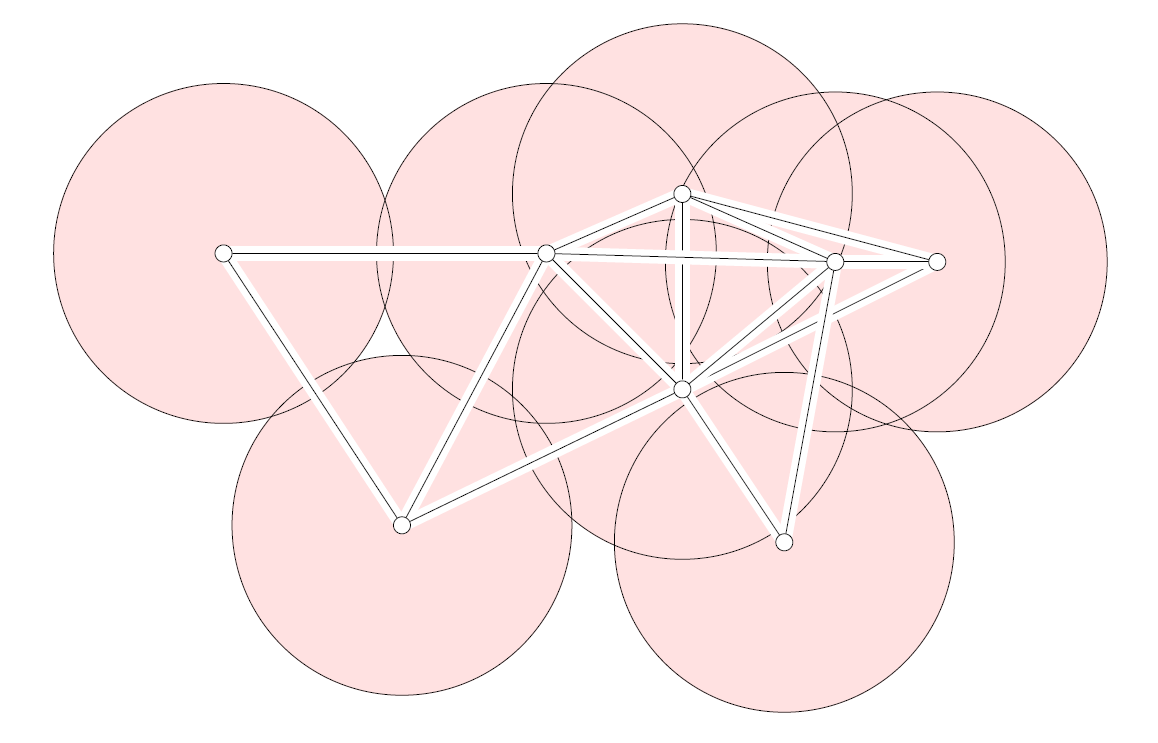
\includegraphics[width=0.5\textwidth]{figures/bg/Cech.png} 
\caption{\v{C}ech complex for a set of nine points and a radius $r$. Source: \cite{edelsbrunner_computational_2010}}
\label{ref:cech}
\end{figure}

We can check that for large enough values of $r$, $\text{\v{C}ech}(r)$ is a simplex of dimension $\text{card }(X)-1$ {\cite[Chapter~3]{bookEH}}, so the \v{C}ech complex is computationally inefficient.

Furthermore, in general, the \v{C}ech complex of a set of points $X \subset \mathbb{R}^d$ does not possess a geometric realization in $\mathbb{R}^d$. Therefore, we will present a construction that resembles the \v{C}ech complex but will be much more favorable from a computational point of view.

\subsubsection*{Vietoris-Rips complex}

\begin{definition}
Let $X \subset \mathbb{R}^d$ be a finite set of points. We call \emph{Vietoris-Rips} complex of $X$ of radius $r$ to the abstract simplicial complex 
\[
\text{VR}(r) = \{\sigma \subseteq  X \mid \textrm{diam } \sigma \leq r\} = \left\{ \{x_0, ..., x_n\} \subseteq  X \mid d(x_i, x_j) \leq r\ \forall i,j\right\}
\]
\end{definition}

We can see in Figure \ref{ref:vr} how the various VR complexes are generated as the radius increases.

\begin{figure}[!ht]
\centering
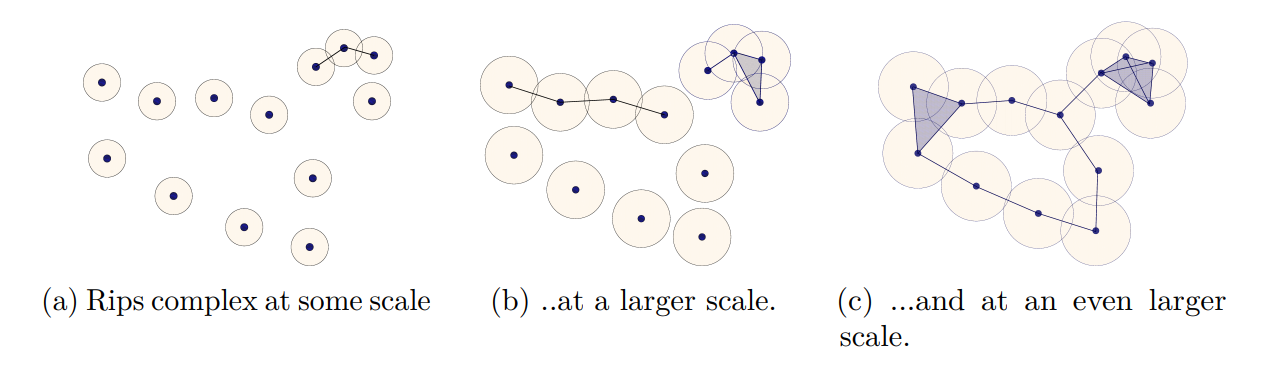
\includegraphics[width=0.9\textwidth]{figures/bg/vr.png} 
\caption{Vietoris-Rips complexes for a set of seven points as we increase the radius from left to right. Source: \cite{ulmer_topological_2019}}
\label{ref:vr}
\end{figure}


Let $\sigma \subset X$, then we remember that the diameter is defined as
\[\textrm{diam } \sigma = \max_{u,v \in \sigma} d(u,v)\,.\]
This observation guarantees that $\sigma \in \text{VR}(r)$ if and only if all its edges are in $\text{VR}(r)$. In other words, $\text{VR}(r)$ is completely determined by its $1$-skeleton. This makes the Vietoris-Rips complex much more efficient than the \v{C}ech complex from the computational point of view. However, as with the \v{C}ech complex, it does not admit a geometric realization in $\mathbb{R}^d$.

On the other hand, the Vietoris-Rips complex is not the nerve of any collection of subsets of $\mathbb{R}^d$. However, the following result guarantees that the VR complex approximates the \v{C}ech complex.

\begin{lemma}[Vietoris-Rips lemma {\cite[Chapter~3]{edelsbrunner_computational_2010}}]
\label{ref:lemaVR}
Let $X \subset \mathbb{R}^d$ be a finite set of points and let $r \geq 0$. Then,
\[
\text{\rm \v{C}ech}(r) \subset \text{\rm VR}(r) \subset \text{\rm \v{C}ech}(\sqrt{2}r)\,.
\]
\end{lemma}








\section{Related work}





\section{Summary}

%\engExpl{It is nice to have this chapter conclude with a summary. For example, you can include a table that summarizes other people's ideas and benefits and drawbacks with each - so as later you can compare your solution to each of them. This will also help you define the variables that you will use for your evaluation.}

\end{document}